% This file is part of the Apogee project.
% Copyright 2014 Melissa Ness and David W. Hogg.

% # short-term to-do
% - draft abstract
% - draft introduction

\documentclass[12pt, preprint]{aastex}
\usepackage{bm}

\input{vc}
\newcommand{\sectionname}{Section}
\newcommand{\documentname}{\textsl{Note}}

\newcommand{\set}[1]{\bm{#1}}
\newcommand{\mean}[1]{\overline{#1}}
\newcommand{\given}{\,|\,}
\newcommand{\teff}{\mbox{$\rm T_{eff}$}}
\newcommand{\feh}{\mbox{$\rm [Fe/H]$}}
\newcommand{\logg}{\mbox{$\rm \log g$}}

\begin{document}

\title{Wavelength-independent stellar parameter determination using data-driven models: The APOGEE example}
\author{
  MKN,
  DWH,
  \&
  HWR}
\date{DRAFT / \gitdate\ / \githash\ / NOT FOR DISTRIBUTION}

% DWH say: Obey A&A abstract rules (ish).
%          They offer good guidance on abstract construction.

\begin{abstract}
In A\&A format: shorten this. move parts to intro.

Aims: We implement a generalised, wavelength independent technique to determine stellar parameters for large datasets, using data-driven models. Our work motivates the importance of having a ``gold standard'' set of stars studied at high resolution, to serve as training data set for stellar surveys. This method has has important applications for homogenising all large surveys and chemical tagging, for which this approach is ideal. \\ %Established standard stars with labels including in [X/Fe], which can be re-observed as part of every new large survey and serve as the training set for the method, has important applications for homogenising all large surveys and chemical tagging, for which this approach is ideal. \\
%
Methods: We use regression techniques to transfer labels from a training set of data to every new star observed, within a given stellar survey. This method is directly transferable between surveys and wavelength regions and relies on a training set of spectra with well defined labels. These labels may include stellar parameters of \teff\, \logg\ and [Fe/H], [$\alpha$/Fe] and individual abundances [X/Fe]. Via this method we characterise how every pixel in a spectra contributes to defining the labels of a star and in doing this, we utilise all of the information within the stellar spectra. \\
Results:  Using the APOGEE dataset and a training set of globular and open clusters observed by APOGEE, we demonstrate that this approach is simple, fast and extremely successful in deriving stellar parameters for APOGEE data. As we exploit every pixel in the spectra, the intrinsic errors in the method are small, which facilitates going to much lower SNR than current approaches. $< $quantify this$>$. As part of this proof of concept we include a catalogue of \teff\, \logg\ and [Fe/H] for 60K stars observed in APOGEE for DR10, including parameters for dwarf as well as giants, which have not been previously reported. \\

\end{abstract}

\section{Introduction}

Challenges of stellar parameter estimation.

In principle there could be data-driven models.

Data-driven models would permit ``label transfer''.
This is especially important if we want optical models to provide labels for infrared surveys (and so on).

APOGEE provides a great data set for exploring these issues. Large homogenous datasets make this possible for the first time. 

Also avoids issue of stellar models once have well characterised set, given any wavelength for calibration and is very fast + generalised. 
issues - cite Meszaros paper for typical implementation. 

We implement this technique as a method to systematically and optimally exploit the information in stellar spectra within large homogeneous datasets.  Our method avoids explicit stellar models and the data itself is the basis of the characterisation. Models are required ab initio and can be implemented at an independent wavelength range, to set the labels for the calibration data.  We apply the primary spectral labels of \teff\, \logg\, [Fe/H] and this process can be extended and applied in N dimensions given well labeled training sets. Calibration sets, of open and globular cluster data, are critical to enable this method which can in principle be implemented with synthetic libraries but this folds in unphysical residuals. We present a general method by using the APOGEE example, characterising the APOGEE spectra and demonstrating how dimensionality of the calibration set can be applied to interpret APOGEE data. 

Motivated by the idea of fingerprinting spectra in the spirt of chemical tagging and developing robust methods that allow the spectra to be mapped in full as a function of its labels. Reverse philosophy to a lot of current techniques were individual lines are the focus, here we disregard what they are and examine impartially. This may reveal information that may not be obvious or otherwise determined. note - Can I find an example of this for the paper? 

%map labels of test set onto the larger set of data

\section{Motivation}

Proof-of-concept: 

We identified a number of regions in APOGEE spectra that serve as relatively temperature and log g insensitive metallicity indicators that can be used to return an [Fe/H] for APOGEE spectra to an accuracy of $<$ 0.15 dex. From this first proof-of-concept phase, we have implemented a regression analysis in pixel or line space, to determine the coefficients or spectral regions that might serve as stellar parameter indicators.  We have a number of aims: (i) characterise the dependence of each pixel on the stellar parameters and identify the key regions of the spectra that are sensitive to the stellar parameters we wish to determine (Teff, log g, [Fe/H], [alpha/Fe]), (ii) use the fits to these regions (using calibration stars) as a baseline to derive the stellar parameters from any given APOGEE spectra and (iii) provide a tool to the community for implementation in the APOGEE-2 project + e.g. Hermes, where stellar parameters can be determined without explicit stellar models. Extensions of this are for individual abundance labels and heuristic index determination.

\section{Data}

read in data; which files, etc.

A training dataset may ideally be one that consists of a set of stars that extend over the parameter range of the observations, in \teff\, \logg\, [Fe/H], [X/Fe] and have their labels derived from high resolution spectral analysis in the optical, where abundance analyses can employ reliable and clean well defined lines and take into account isotopic and hyperfine splitting effects for individual abundances. The training set we employ for this data driven analysis is that of the globular and open cluster data observed by APOGEE for calibration of their abundance pipeline \citep{Mesaroz2013}. This training data set is comprised of 20 open and globular clusters, which span stellar parameter ranges of 3500 $<$ \teff\ $<$ 5300, 0 $<$ \logg 5 and --2.5 $<$ [Fe/H] $<$ 0.45. We adopt the ``ASPCAP corrected'' stellar parameters of each of these stars in the training set as our tags for the stars; this nominally ensures that we are on the same calibration as APOGEE for stellar parameters. The corrections made by APOGEE for the cluster data are applied to the direct output of the ASPCAP pipeline based on a temperature calibration to the infrared flux method \citep{Gonzalez2009} ,a \logg\ correction from the offset between ASCAP results and Kepler results for common stars and [Fe/H] offsets from the output of ASCAP versus the literature value of each cluster.  The APOGEE corrections that they determine are valid only for stars with \logg\ $<$ 3.5 and are not implemented for the dwarfs. 

These corrections place the giants in the cluster stars on or near the iscohrones (see Figures 7 and 8 in Meszaros et al., (2013)). We  also correct the ASPCAP dwarf cluster spectra to the infrared flux value of \citep{Gonzalez2009} which is small at their temperatures, offset the metallicities of these stars by the difference between the mean value from the ASPCAP pipeline and the literature values of the clusters from Meszaros et al., 2013 and shift the \logg\ values of the stars to their nearest positions on the isochrone, moving the stars vertically without adjusting the other calibrated parameters. \textit{actually I have not done this yet - most important will be logg other changes are small}.

The analysis in \citet{Meszaros2013} is restricted to giants and stars with SNR $>$ 70, determined to be the minimum for reliable stellar parameters. Our method is calibrated across dwarfs and giants and can return reliable stellar parameters to a SNR of XXX, with an intrinsic scatter of x,y,z in \teff, \logg, \feh. 

- See Figure X for the training set histograms of t, g, feh. 

For our regression analysis, where pixels are directly compared between stars in the training set, it is essential to have a robust continuum normalisation that will ensure pixels are compared fairly between stars of different parameters. We therefore implement a weighted median method, but instead of returning the central tendency we consider the 85\% quantile, returning the typical continuum level and effectively excluding outliers, considered over intervals of 50\AA of the spectra. This provides a consistent normalisation across the spectra. Three typical spectra are shown in Figure X demonstrating this normalisation routine is effective. Similarly to the training set, all data input to the regression must be treated in the same way with the same continuum normalisation.
\textit{ note - need to consider coolest stars and also high signal to noise and may need to adjust quantile for this. }

re-continuum-normalize; how?

demonstrate that the normalization is good.

meta-data on cluster stars; why do we believe it; table - just reference Meszaros 2013 for this or we are repeating information. 

\section{Spectral model}

The model is that the observed, continuum-normalized spectrum, at each
wavelength, can be explained as a linear combination of real-valued
``tags'', or a linear combination of functions of those tags.
Here the tags will be things like effective temperature $\teff$,
logarithmic surface gravity $\logg$, and metallicity $\feh$.
Additionally, the model is that at each wavelength, the observed
spectrum will deviate from the linear combination by some additive
noise contribution, some of which comes from photon noise and
sky-subtraction noise and other instrumental contributions, and some
of which is an intrinsic scatter, presumed independent at each
wavelength.
The model is built using ``training data'' (with known tags) and then
used to tag (or infer tags for) the ``test data''.

In the training data there will be $N$ spectra $n$, each of which has
a continuum-normalized flux measurement $y_{n\ell}$ at wavelength
$\lambda_\ell$, and an associated uncertainty variance
$\sigma_{n\ell}^2$ from finite photon counts and instrumental effects.
If there are missing flux values in the training data, these can be
handled by setting variances to something very large (or inverse
variances to something very small).
Each of the training spectra $n$ has $K$ tags $x_{nk}$, each of which
is (for now) presumed to have negligible uncertainty.
The general model is
\begin{eqnarray}
y_{n\ell} &=&
 Y(\set{x}_n\given\set{\theta}_\ell) + [s_\ell^2 + \sigma_{n\ell}^2]^{1/2}\,\xi_{n\ell}
\label{eq:model}\\
\set{x}_n &\equiv& [x_{n1}, x_{n2}, \cdots, x_{nK}]
\quad,
\end{eqnarray}
where $Y()$ is some (possibly complicated) function of the full set
of $K$ tags, $\set{x}_n$ is a vector or blob of the $K$ tags for spectrum $n$,
$\set{\theta}_\ell$ is the set of parameters controlling the
function $Y()$ at wavelength $\lambda_\ell$, $s_\ell^2$ is an
intrinsic variance for the model at wavelength $\lambda_\ell$, and
$\xi_{n\ell}$ is a Gaussian random number with zero mean and unit
variance.
That is, we have assumed that the noise is Gaussian, zero mean, and
independent for every measurement.
This model leads to the single-pixel log-likelihood function
\begin{eqnarray}
\ln p(y_{n\ell}\given\set{\theta}_\ell,s_\ell^2) &=&
 -\frac{1}{2}\frac{[y_{n\ell} - Y(\set{x}_n\given\set{\theta}_\ell)]^2}{s_\ell^2 + \sigma_{n\ell}^2}
 -\frac{1}{2}\ln(s_\ell^2 + \sigma_{n\ell}^2)
 -\frac{1}{2}\ln 2\pi
\label{eq:like1}\\
\set{x}_n &\equiv& [x_{n1}, x_{n2}, \cdots, x_{nK}]
\quad.
\end{eqnarray}
Since all the spectra and pixels are treated as independent, each
wavelength $\lambda_\ell$ can have its parameters
$[\set{\theta}_\ell,s_\ell^2]$ inferred independently, and all the
individual-spectra log-likelihoods can be added together to make
\begin{eqnarray}
\ln p(\set{y}_\ell\given\set{\theta}_\ell,s_\ell^2) &=&
 \sum_{n=1}^N \ln p(y_{n\ell}\given\set{\theta}_\ell,s_\ell^2)
\label{eq:like}\\
\set{y}_\ell &\equiv& [y_{1\ell}, y_{2\ell}, \cdots, y_{N\ell}]
\quad,
\end{eqnarray}
where $\set{y}_\ell$ is the vector of spectral flux values for
the $N$ objects all at wavelength $\lambda_\ell$.
We can set the parameters $[\set{\theta}_\ell,s_\ell^2]$ either by
optimizing the likelihood (\ref{eq:like}) or by applying priors and
performing some kind of probabilistic inference (with, say, Markov
Chain Monte Carlo techniques).
Here we will optimize for now.

In this \sectionname, we are treating the function parameters
$\set{\theta}_\ell$ and the scatter $s_\ell^2$ as free parameters, and the
tags $x_{nk}$ as fixed.
The likelihood function (\ref{eq:like}) is presented as being a
function of these free parameters.
In the next \sectionname, the tables will turn, and we will treat the
function parameters $\set{\theta}_\ell$ and scatter $s_\ell^2$ as fixed and
the tags $x_{nk}$ as parameters.
The difference is that here we are treating the training data as
having perfectly known tags, and later we will be inferring tags for
new spectra.

The simplest spectral model is that in which the functions $Y()$ are
linear in the tags:
\begin{eqnarray}
Y(\set{x}_n\given\set{\theta}_\ell) &=&
 a_{\ell 0} + \sum_{k=1}^K a_{\ell k}\,[x_{nk} - \mean{x_k}]
\label{eq:linear}\\
\set{x}_n &\equiv& [x_{n1}, x_{n2}, \cdots, x_{nK}]
\\
\set{\theta}_\ell &\equiv& [a_{\ell 0}, a_{\ell 1}, \cdots, a_{\ell K}]
\quad ,
\end{eqnarray}
where the $a_{\ell k}$ are linear coefficients, and
the $\mean{x_k}$ are offsets (possibly means of the training data) to
keep the model ``pivoting'' around a reasonable point in tag space.
This linear-in-tags form (\ref{eq:linear}) has many useful and
excellent properties.
The first is that optimization of the model, at fixed scatter
$s_\ell^2$ is a pure linear-algebra operation (weighted least
squares); simultaneous optimization of all the parameters
$[\set{\theta}_\ell,s_\ell^2]$ is only nonlinear in the $s_\ell^2$
parameter.
The second is that the tag inference (label transfer; described in the
next Section) on the test data will have a very simple form.
The third is that the coefficients $a_{\ell 0}$, seen as a discrete
function of wavelength $\lambda_\ell$, can be seen as an estimate of
the \emph{mean spectrum} (provided that the offsets $\mean{x_k}$ are
the mean tag values over the $N$ training spectra); and the
coefficients $a_{\ell k}$ can be seen as the mean first derivatives of
the expected spectrum with respect to each of the $k$ tags, estimated
over the range of the training data.

The results for the linear-in-tags model (\ref{eq:linear}) are shown
in Figures~XXX through YYY.  They show... departures from
linearity... outliers...

...what are we doing about outliers?  If anything?  Perhaps in discussion too...

...Of course weak lines might be closer to linear... what happens when
we restrict to weak lines?..

...is this a good model?  No; how do we know?

The (perhaps) second-simplest spectral model is that in which the
functions $Y()$ are quadratic in the tags:
\begin{eqnarray}
Y(\set{x}_n\given\set{\theta}_\ell) &=&
 a_{\ell 0} + \sum_{k=1}^K a_{\ell k}\,[x_{nk} - \mean{x_k}]
 + \sum_{k=1}^K \sum_{k'=k}^K a_{\ell kk'}\,[x_{nk} - \mean{x_k}]\,[x_{nk'} - \mean{x_{k'}}]
\label{eq:quadratic}\\
\set{x}_n &\equiv& [x_{n1}, x_{n2}, \cdots, x_{nK}]
\\
\set{\theta}_\ell &\equiv& [a_{\ell 0}, a_{\ell 1}, \cdots, a_{\ell K},
                            a_{\ell 11}, a_{\ell 12}, \cdots, a_{\ell KK}]
\quad ,
\end{eqnarray}
where the $a_{\ell k}$ and $a_{\ell kk'}$ are linear coefficients, and
the $\mean{x_k}$ are offsets (possibly means of the training data) to
keep the model ``pivoting'' around a reasonable point in tag space.
This quadratic-in-tags form (\ref{eq:quadratic}) is similar to and
different from the linear-in-tags form (\ref{eq:linear}) in a number
of ways.
It is still the case that optimization of the model, at fixed scatter
$s_\ell^2$ is a pure linear-algebra operation (weighted least
squares).
However, tag inference (described in the next Section) on the test
data will no longer be simple; it will now require non-linear
optimization.
The coefficients $a_{\ell 0}$ can still be seen as an estimate of the
\emph{mean spectrum} (provided that the offsets $\mean{x_k}$ are the
mean tag values); the first-order coefficients $a_{\ell k}$ can still
be seen as first derivatives of the expected spectrum with respect to
each of the $k$ tags, but now evaluated at the mean spectrum; the
second-order coefficients $a_{\ell kk'}$ can now be seen as mean
second derivatives of the expected spectrum with respect to pairs of
tags $k$ and $k'$.

The results for the quadratic-in-tags model (\ref{eq:linear}) are shown
in Figures~XXX through YYY.  They show... departures from
linearity... outliers... is it really a better model?..

\section{Parameter estimation}

In the previous \sectionname, we built data-driven spectral models
from training data.
These models have the property that, given tags, they can be used to
predict continuum-normalized flux, up to observational and intrinsic
scatter.
In this \sectionname, we are going to solve the inverse problem; we
are going to presume that we have spectra, but we don't have tags.
In this case, we will use inference to obtain tags for the untagged
spectra.
These untagged spectra will be referred to as the ``test data'' in
what follows.

In the test data there will be $M$ spectra $m$, each of which---as in
the training data---has a continuum-normalized flux measurement
$y_{m\ell}$ at each of $L$ wavelengths $\lambda_\ell$, and an
associated observational uncertainty variance $\sigma_{m\ell}^2$.
Again, if there are missing flux values in the test data, these can be
handled by setting variances to something very large.
The difference between the training data and the test data is that the
test data do not (yet) have known tags $x_{mk}$; we are going to infer
these.

Just as in the previous \sectionname, our model is given in
equation~(\ref{eq:model}).
This model leads to the same likelihood function given in
equations~(\ref{eq:like1}) and (\ref{eq:like}), but this time seen as
being functions not of the function parameters $\set{\theta}_\ell$ and
scatter $s_\ell^2$ but instead as functions of the \emph{tags}
$x_{mk}$:
\begin{eqnarray}
\ln p(y_{m\ell}\given\set{x}_m) &=&
 -\frac{1}{2}\frac{[y_{m\ell} - Y(\set{x}_m\given\set{\theta}_\ell)]^2}{s_\ell^2 + \sigma_{m\ell}^2}
 -\frac{1}{2}\ln(s_\ell^2 + \sigma_{m\ell}^2)
 -\frac{1}{2}\ln 2\pi
\\
\ln p(\set{y}_m\given\set{x}_m) &=&
 \sum_{\ell=1}^L \ln p(y_{m\ell}\given\set{x}_m)
\label{eq:taglike}\\
\set{x}_m &\equiv& [x_{m1}, x_{m2}, \cdots, x_{mK}]
\\
\set{y}_m &\equiv& [y_{m1}, y_{m2}, \cdots, y_{mL}]
\quad,
\end{eqnarray}
where the likelihood functions are given as a function of tags now,
the sum is now over the full set of $L$ wavelengths
$\lambda_\ell$, and the vector $\set{y}_m$ is the vector of fluxes from
spectrum $m$ for all $L$ wavelengths $\lambda_\ell$.
These likelihood functions effectively assume that the function
parameters $\set{\theta}_\ell$ and scatters $s_\ell^2$ are all known (from
the training data).
New tags $x_{mk}$ for object $m$ can be obtained either by maximizing
the likelihood function (\ref{eq:taglike}), or else by applying priors
and performing probabilistic inference.
Here we will optimize for now.

When we use the simple linear-in-tags form (\ref{eq:linear}) for the
mean model $Y()$, the optimization to obtain maximum-likelihood tags
(given parameters $[\set{\theta}_\ell, s_\ell^2]$) is simple linear
least-square fitting.
This optimization is obtained by straightforward linear algebra on the
spectral pixels $y_{m\ell}$, and standard frequentist confidence
intervals can be obtained similarly.
Results for the linear-in-tags model are shown in Figures~XXX through
YYY.

When we use the quadratic-in-tags form (\ref{eq:quadratic}) for the
mean model $Y()$, there is no simple linear-algebra operation that
optimizes the likelihood.



...why is linear so much easier than quadratic or GP?  Methodological details

...leave-one-cluster-out cross-validation

...application to some example APOGEE targets and comparison to ASPCAP

\section{Discussion}

...Did it work and etc?  Weak lines, order, etc.

...Structure of the problem:
We \emph{didn't} do the standard thing of ``just'' asking the fluxes to predict the tags.
We asked the tags to predict the fluxes, and then once that worked, we found the tags that predict the fluxes for other stars.
This structure permits us to respect the noise model (noisy, heteroskedastic fluxes).

...Limitations of the training sample.  Mainly its smallness!

...Limitations of assuming the training sample has perfect tags.

...Linear (or quadratic) model is a very rigid assumption; obviously wrong.
Generalize to a GP at every wavelength.

...Limitations of working at one wavelength at a time in model-building.

...Limitations of the inference procedure at tagging time

...What would the fully probabilistic generalization look like?
It would involve generating samples at training time.
Then use all samples at tagging time.
Produce also a sampling in the tags.
Would have the great advantage that we could use partially or noisily tagged objects in training!
Would require priors on everything.

...Next-generation applications of these methods, esp chemical tagging

\section{Draft Figures}

\begin{figure}[h!]
  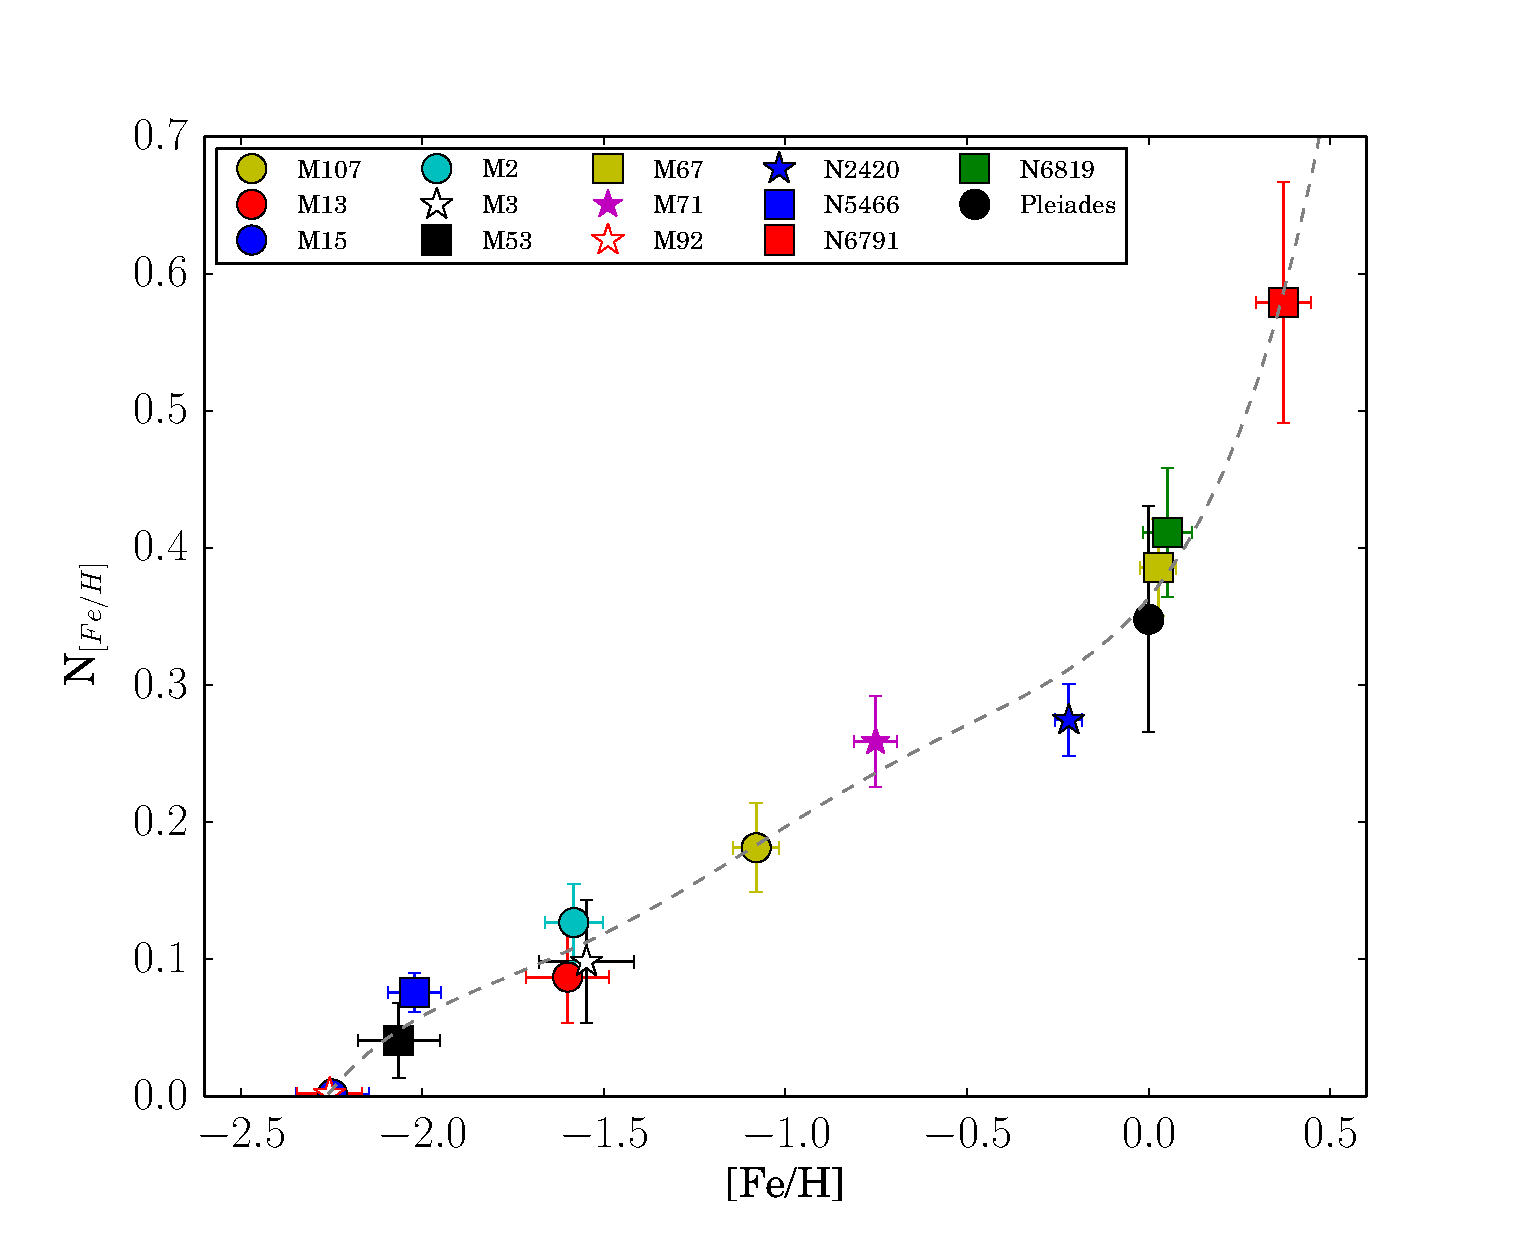
\includegraphics[width=\hsize]{./plots/metals_index.eps}
\caption{Proof of concept/motivating background: The calibration of metallicity of the clusters using an index N$_{[Fe/H]}$, derived from 30 $\AA$ (1\%) of the spectra, using 5 $\times$ lines determined to be [Fe/H]-sensitive and relatively \logg\ and \teff\ insensitive. The error bars represent the dispersion of the points
  around the mean. In total about 450  stars have been used for this
  calibration: M~107 (18 stars), M~13 (71 stars), M~15 (11 stars), M~2
  (19 stars), M~3 (73 stars), M~53 (16 stars), M~67 (24 stars), M~71
  (6 stars), M~92 (48 stars), NGC~2420 (9 stars), NGC~5466 (8 stars),
  NGC~6791 (23 stars), NGC~6819 (29 stars), and Pleiades (75 stars)  \textbf{Note I am missing some clusters in this I should add them in} .}
\label{fig:index}
\end{figure}

\begin{figure}[h!]
  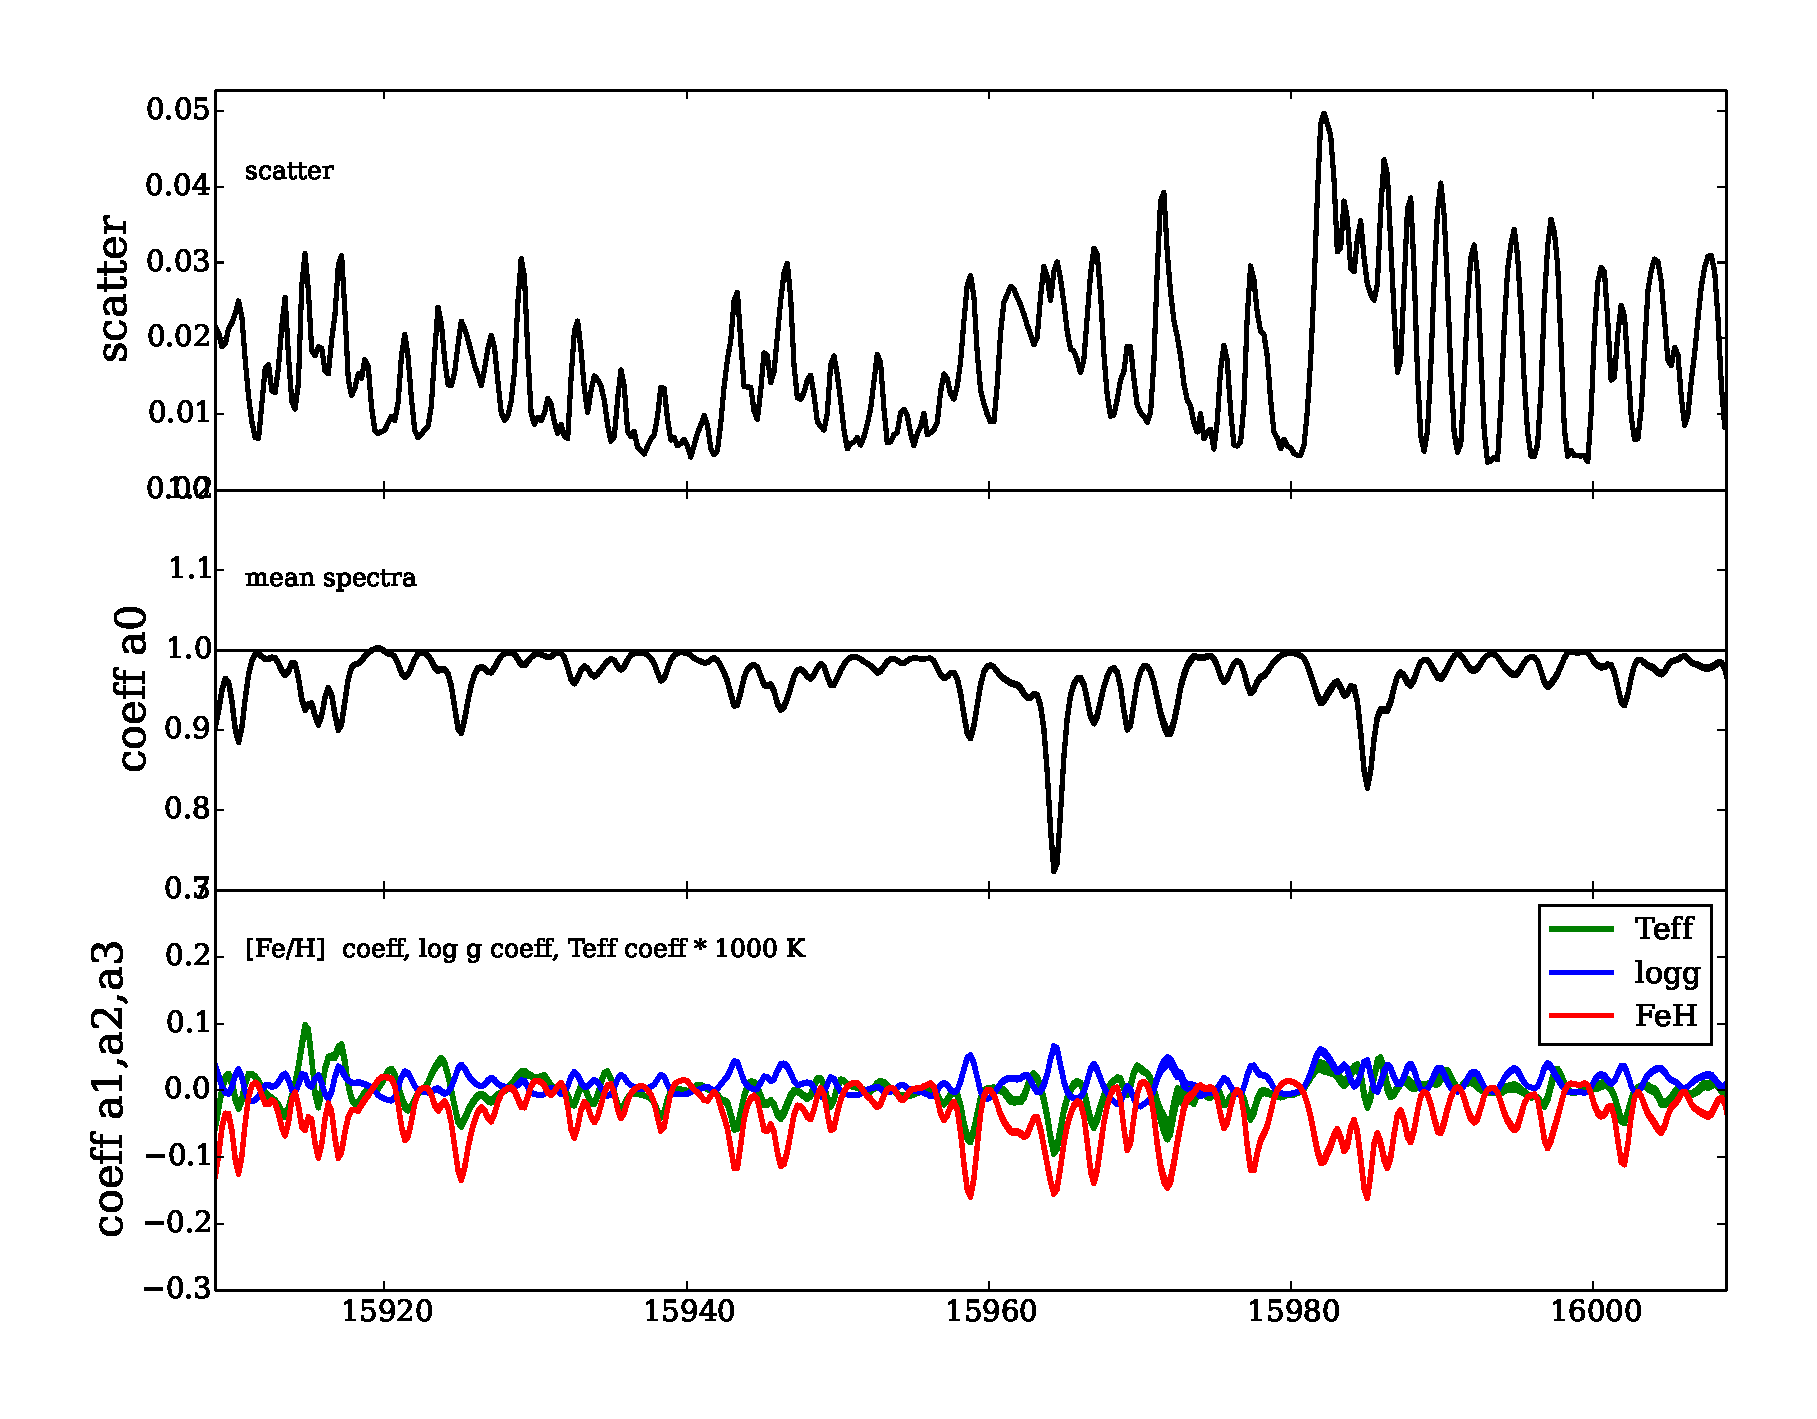
\includegraphics[width=\hsize]{./plots/R1_example.eps}
\caption{The results from the linear regression across at 100 $\AA$ sample region of spectra. The top panel shows the scatter at each wavelength, the centre panel shows the mean spectrum derived from the training set and the bottom panel shows the coefficients fit in each dimension, \teff\, \logg\, [Fe/H]. Given additional labels it will be possible to include more dimensionality, for example [$\alpha$/Fe] and [X/Fe].}
\label{fig:fits}
\end{figure}

\begin{figure}[h!]
  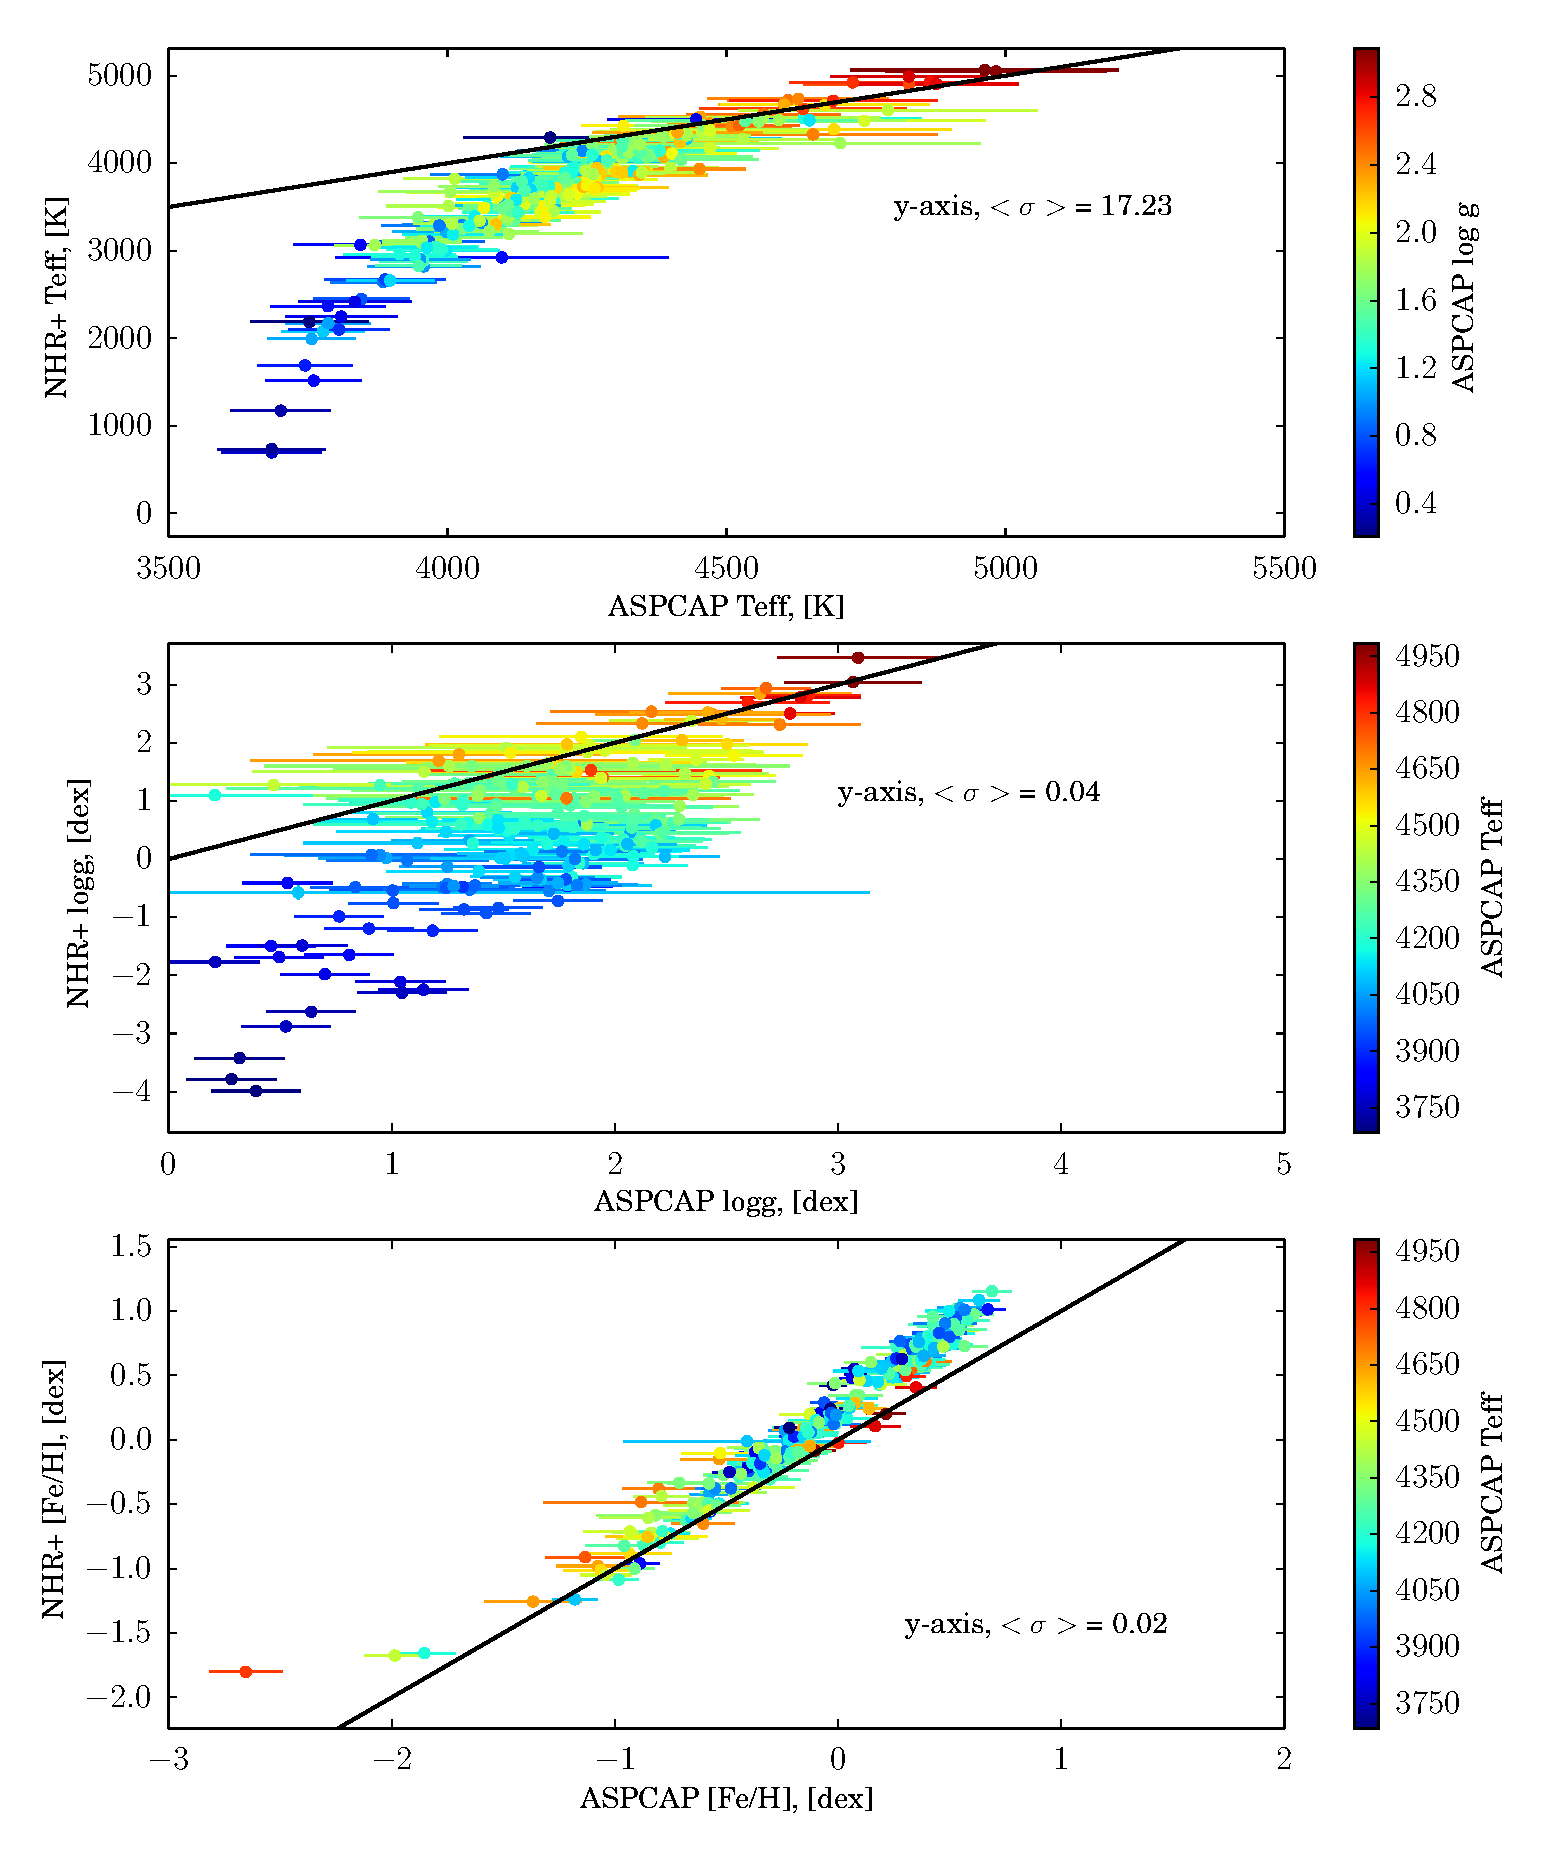
\includegraphics[width=\hsize]{./plots/fits_all3.eps}
\caption{\small{Comparison of our method with ASCAP results for the field 4332 (l,b) = (0,-5$^\circ$). The tight correlation in \teff\ and [Fe/H] suggests that these labels in the training set are very good. There is more scatter in the \logg\ panel that may not represent bad labels in the training set and therefore may not be accounted for in the non-linear model. Comparing Figure \ref{fig:index} with the bottom panel, the discontinuity at ASCAP [Fe/H] $\sim$ 0, is due to the non-linear behaviour of the [Fe/H] which is seen in the index, but which is not captured in our linear model (see Figure \ref{fig:index}).}}
\label{fig:cal}
\end{figure}

\begin{figure}[h!]
  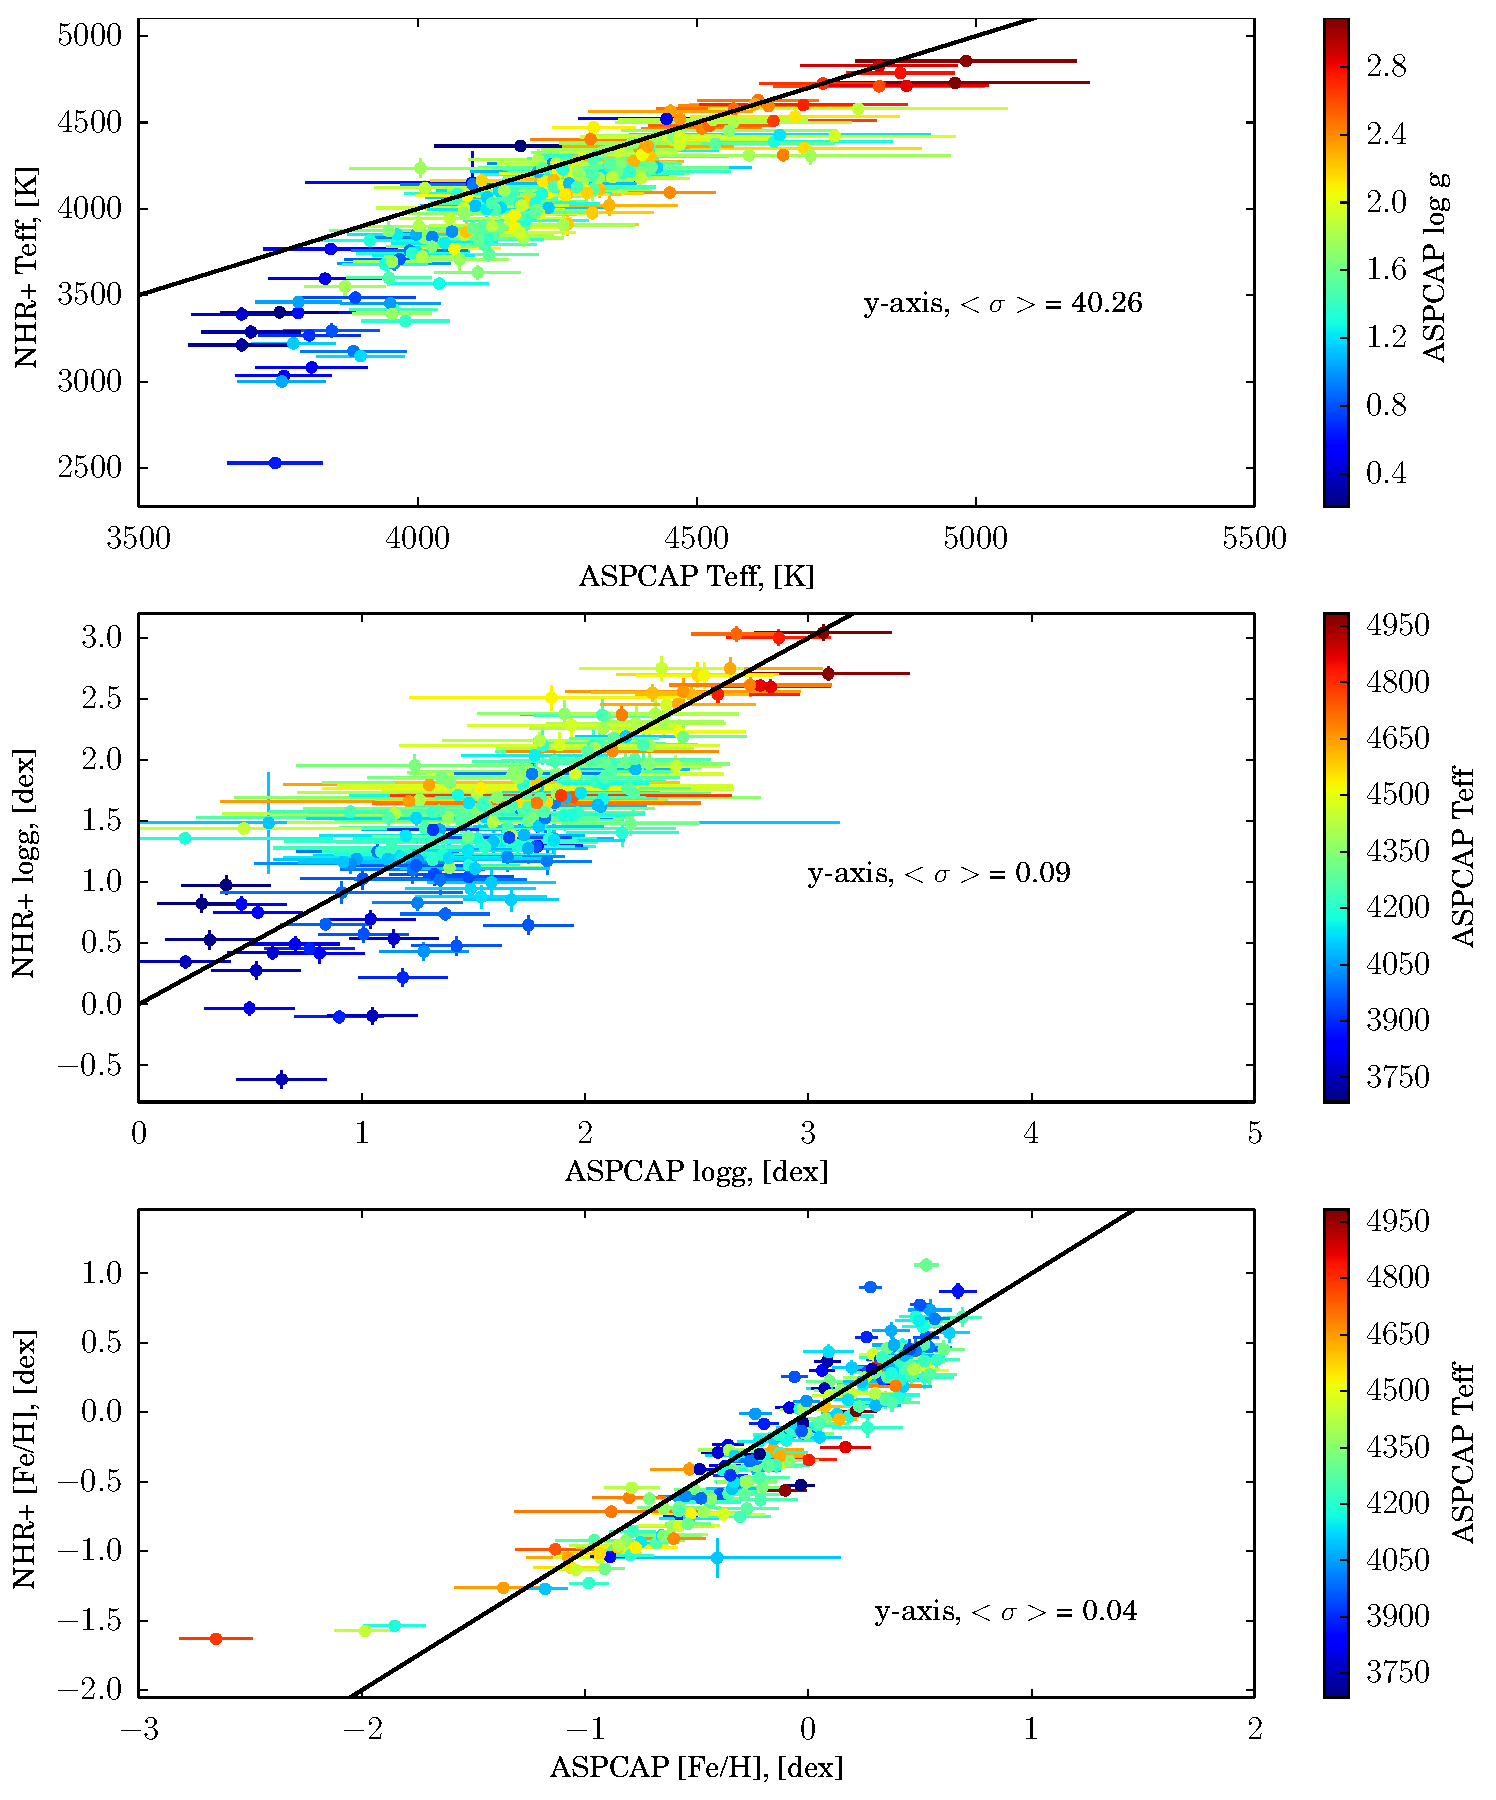
\includegraphics[width=\hsize]{./plots/fits_all3_continuumcut.eps}
\caption{\small{Comparison of our method with ASCAP results for the field 4332, using a continuum cut to select for the weak features and to exclude stronger lines. This was done to avoid the known effect of non-linearities in stronger absorption features and the cut implemented for this figure is 0.935 $<$ flux $<$ 0.99, equivalent to about 50\% of the flux of the median spectra. (note: both bounds are necessary to achieve these fits). Using weaker lines, a linear model is demonstrated to be a reasonably good model for the data. The scatter increases by about a factor of 2 in each dimension by adopting this continuum cut. }}
\label{fig:cut1}
\end{figure}

\begin{figure}[h!]
  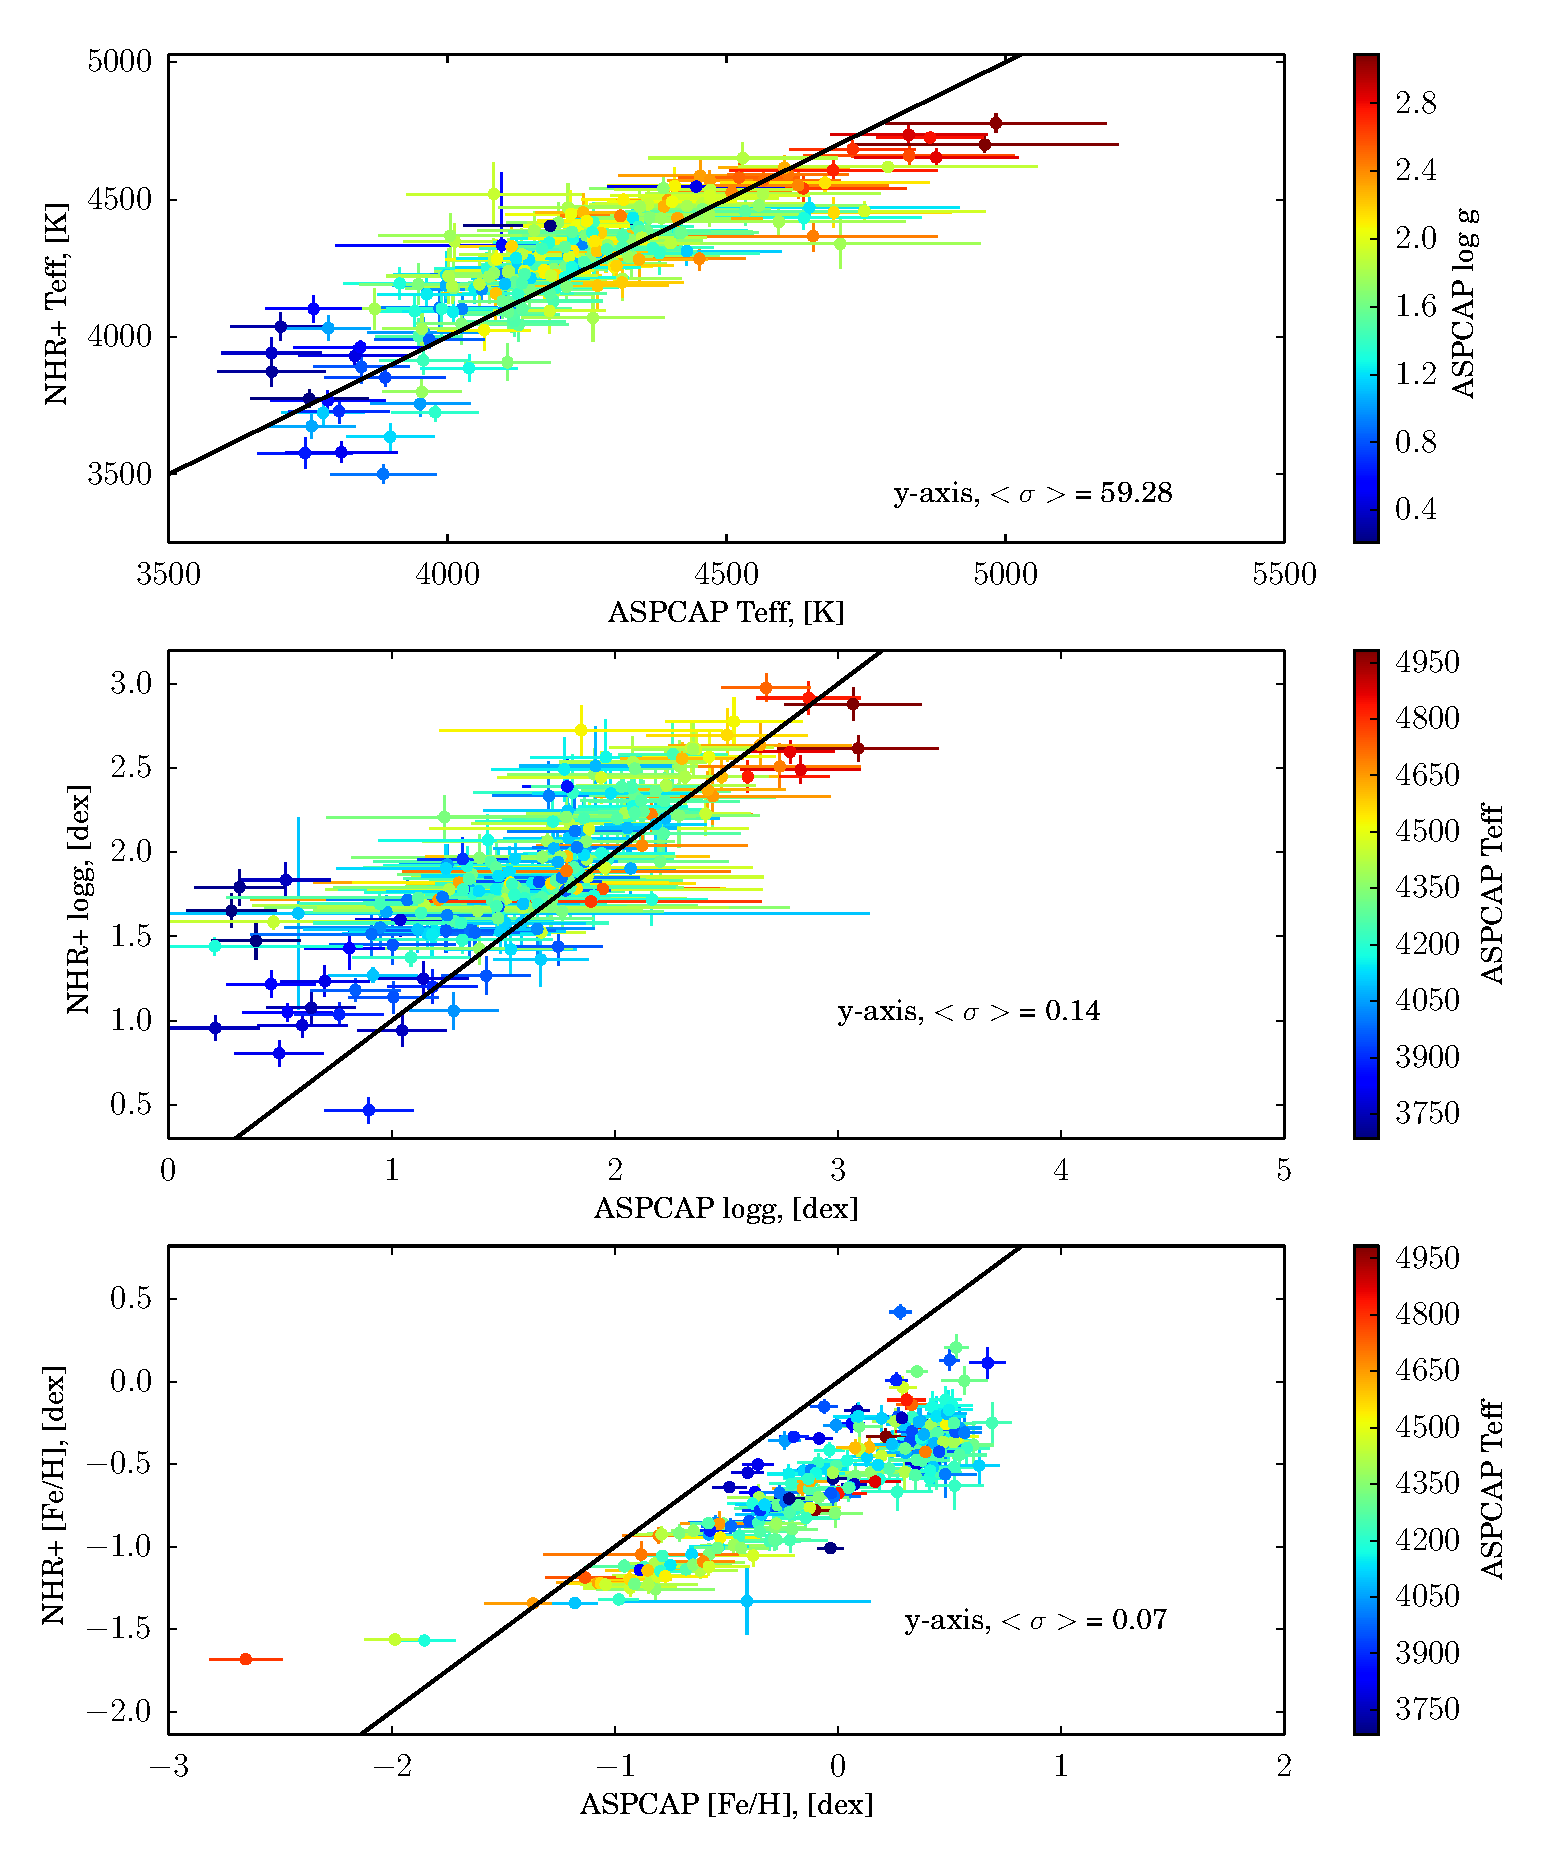
\includegraphics[width=\hsize]{./plots/fits_all3_continuumcut2.eps}
\caption{\small{As for figure \ref{fig:cut1} but using a tighter continuum cut of 0.95 $<$ flux $<$ 0.99. This demonstrates that the information for the [Fe/H] characterisation is lost at this tighter cut on the continuum, it suggests that the sensitivity of the spectra to log g is lower at the low temperature end of the spectra and the information in temperature is fairly well recovered using a linear scale for this cut in flux. } }
\label{fig:cut2}
\end{figure}

\begin{figure}[h!]
  \includegraphics[width=\hsize]{./plots/coeff_map.eps}
\caption{per pixel scaled residuals for stars ordered in [Fe/H], from the most metal poor at the bottom to the most metal rich at the top}
\label{fig:coeff}
\end{figure}

\begin{figure}[h!]
  \includegraphics[width=\hsize]{./plots/chi_map.eps}
\caption{Spectral Fingerprints for calibration clusters showing the chi2 coefficients for each star at each pixel separated into clusters from the most metal rich to the most metal poor (divided by horizontal lines) 
\textbf{To do; put clusters + [Fe/H] on other y-axis)}}
\label{fig:DNA}
\end{figure}

\begin{figure}[h!]
  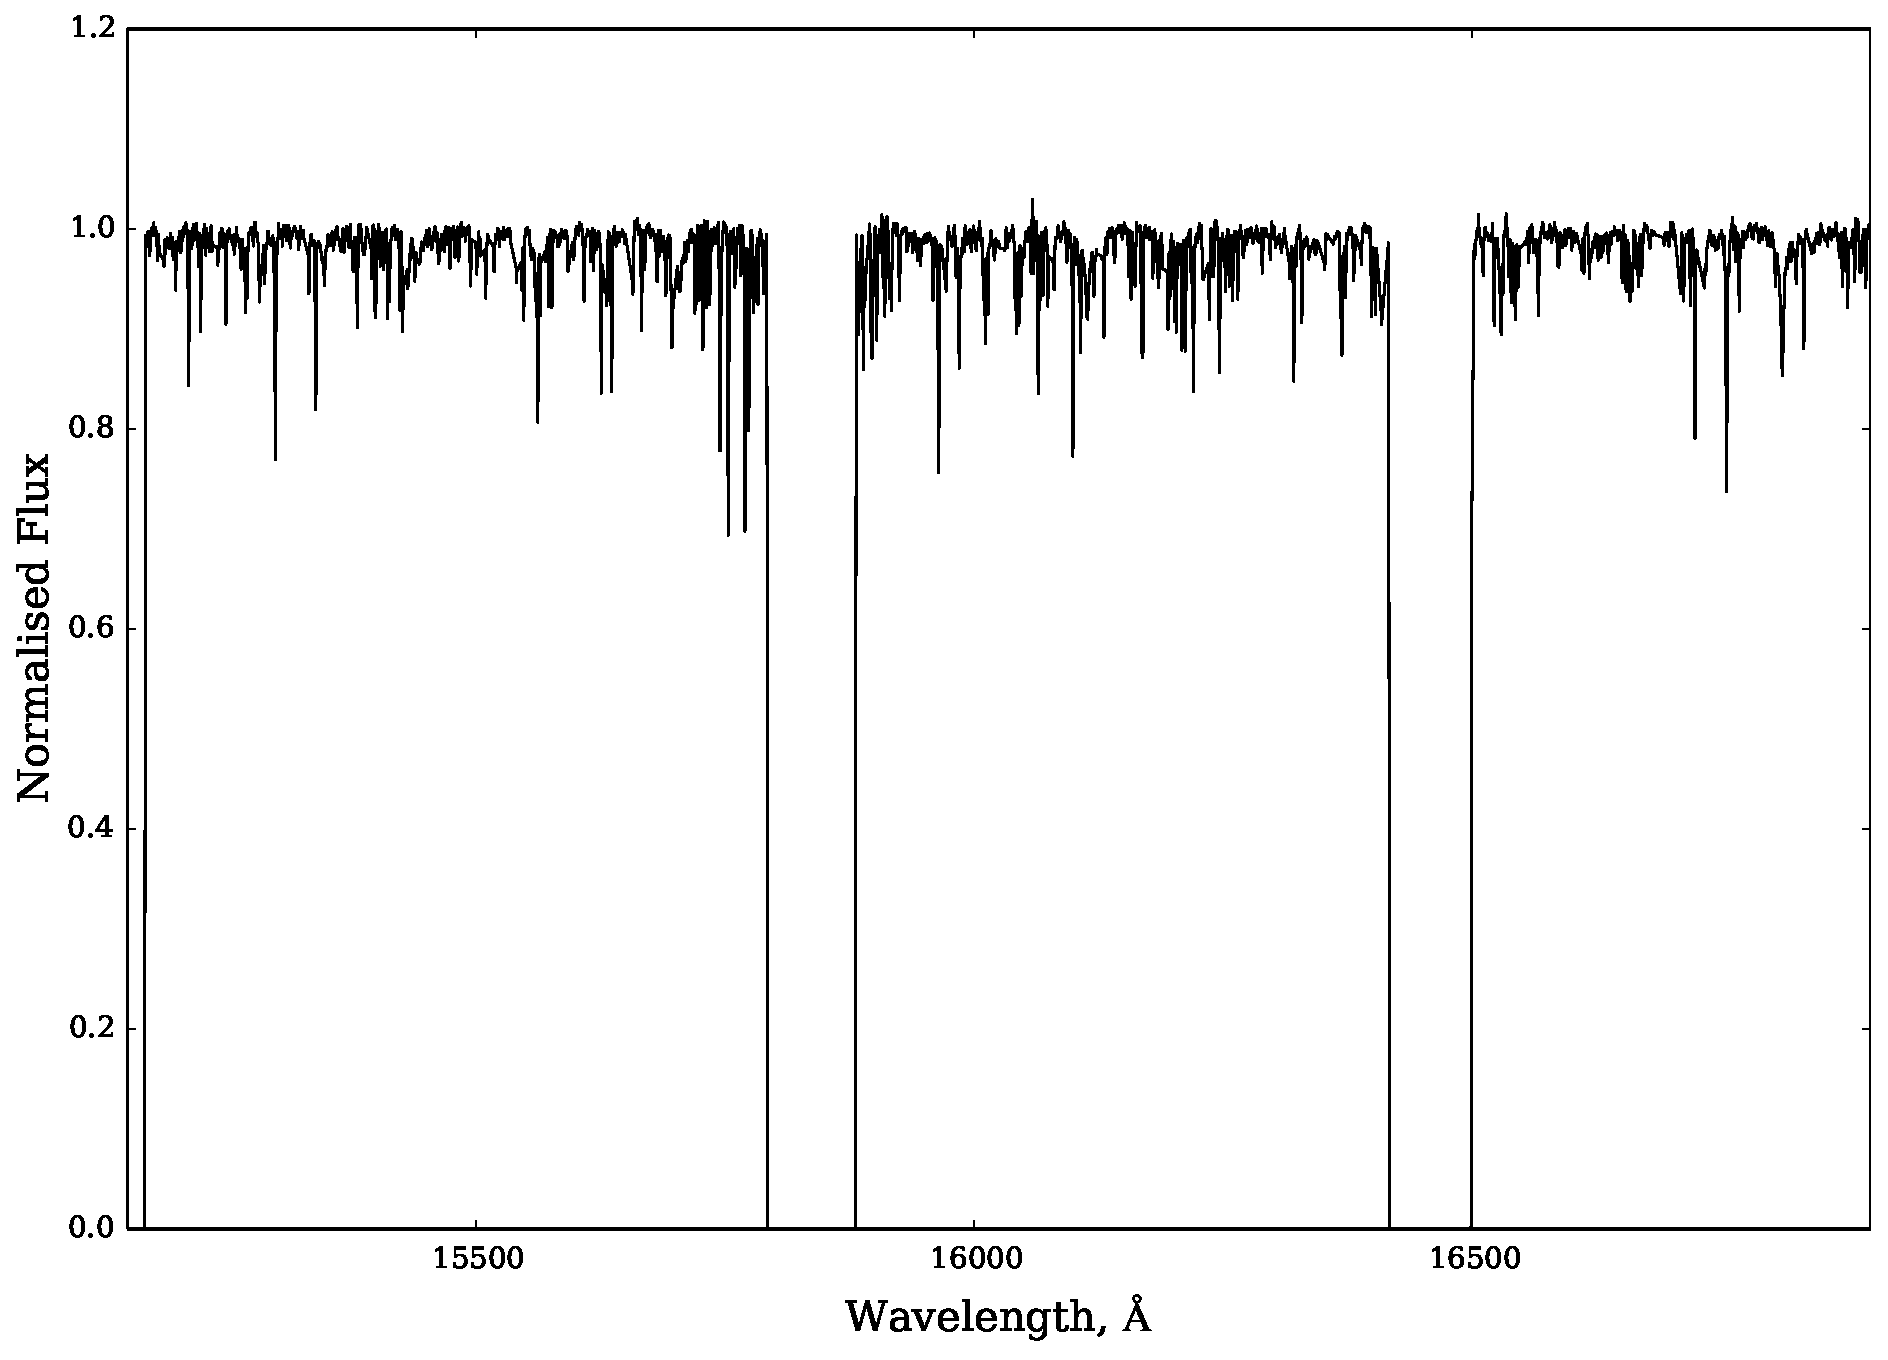
\includegraphics[width=\hsize]{./plots/normed_300.eps}
\caption{Sample continuum normalised spectra}
\label{fig:DNA}
\end{figure}

\begin{figure}[h!]
  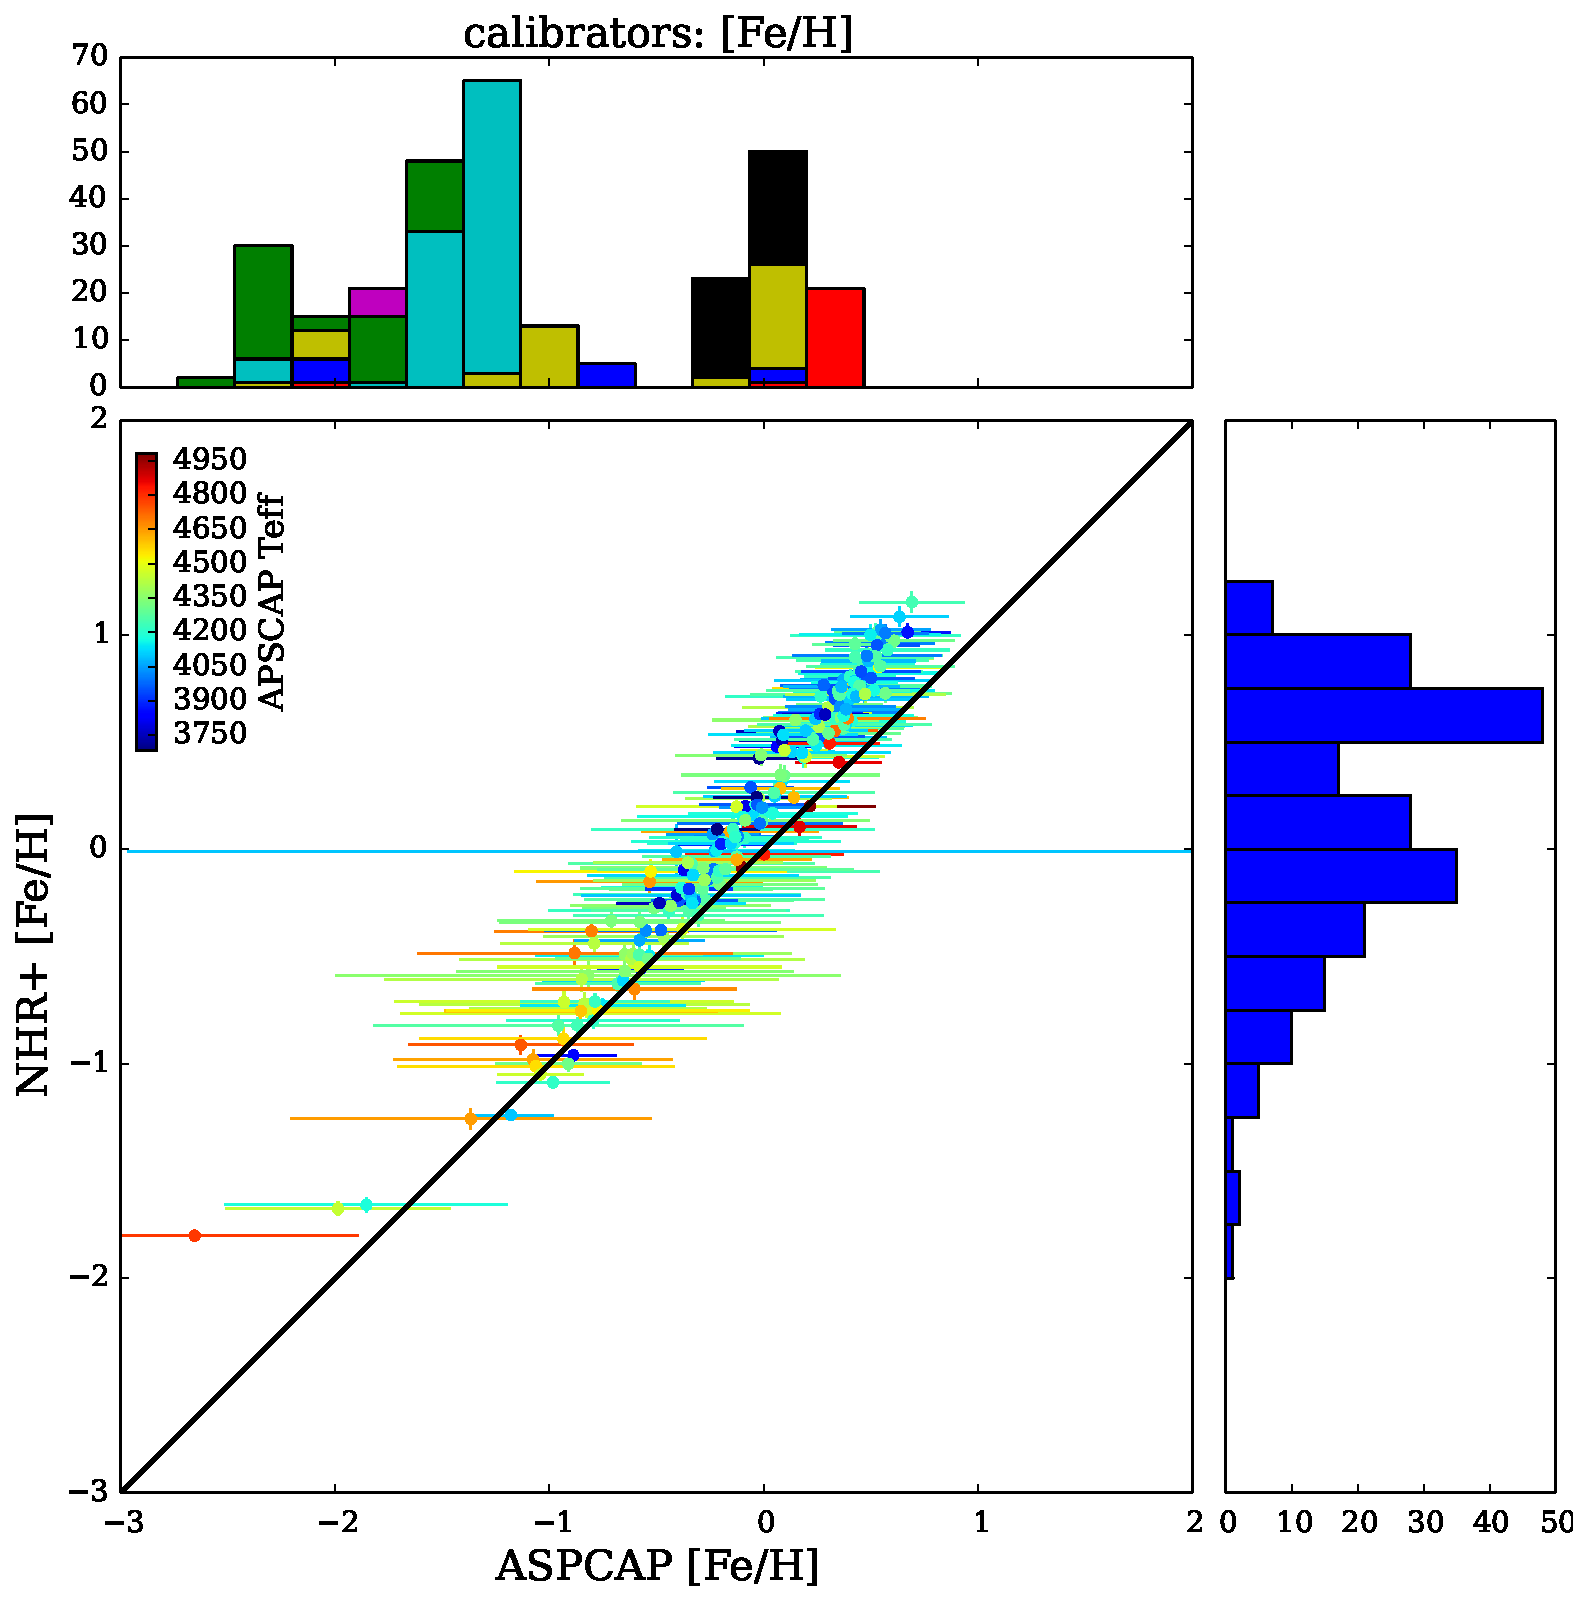
\includegraphics[width=\hsize]{./plots/cal_feh.eps}
\caption{\textbf{Need to change these to stack the histograms}: Showing the spread of calibration stars in training set across [Fe/H] - sparse sampling is not a problem in the centre for this label}
\label{fig:cal_feh}
\end{figure}

\begin{figure}[h!]
  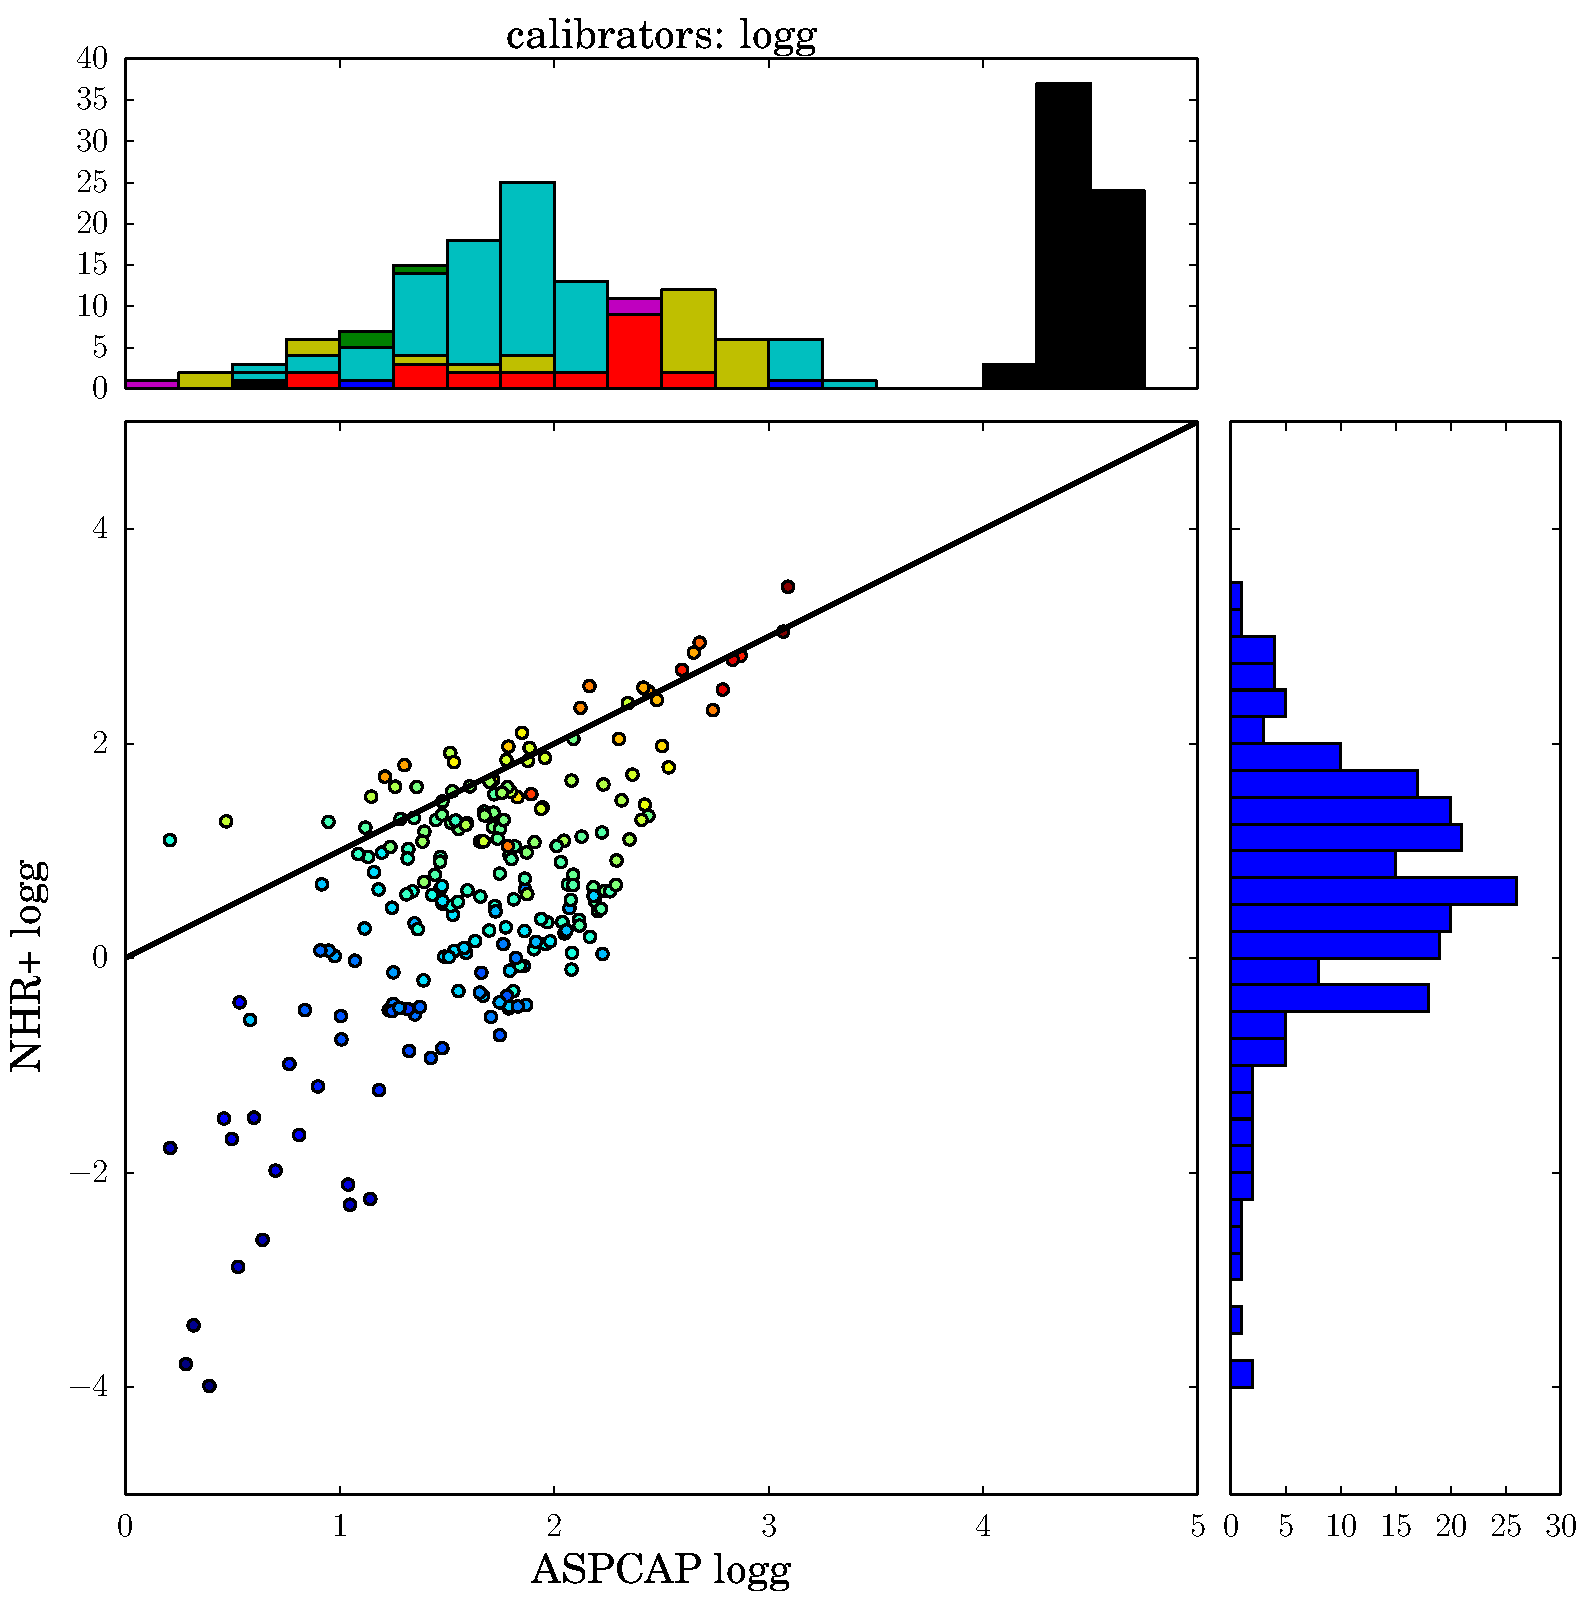
\includegraphics[width=\hsize]{./plots/cal_logg.eps}
\caption{Showing the spread of calibration stars in training set across log g ; missing sub giant stars - would be very good to have these }
\label{fig:cal_g}
\end{figure}

\begin{figure}[h!]
  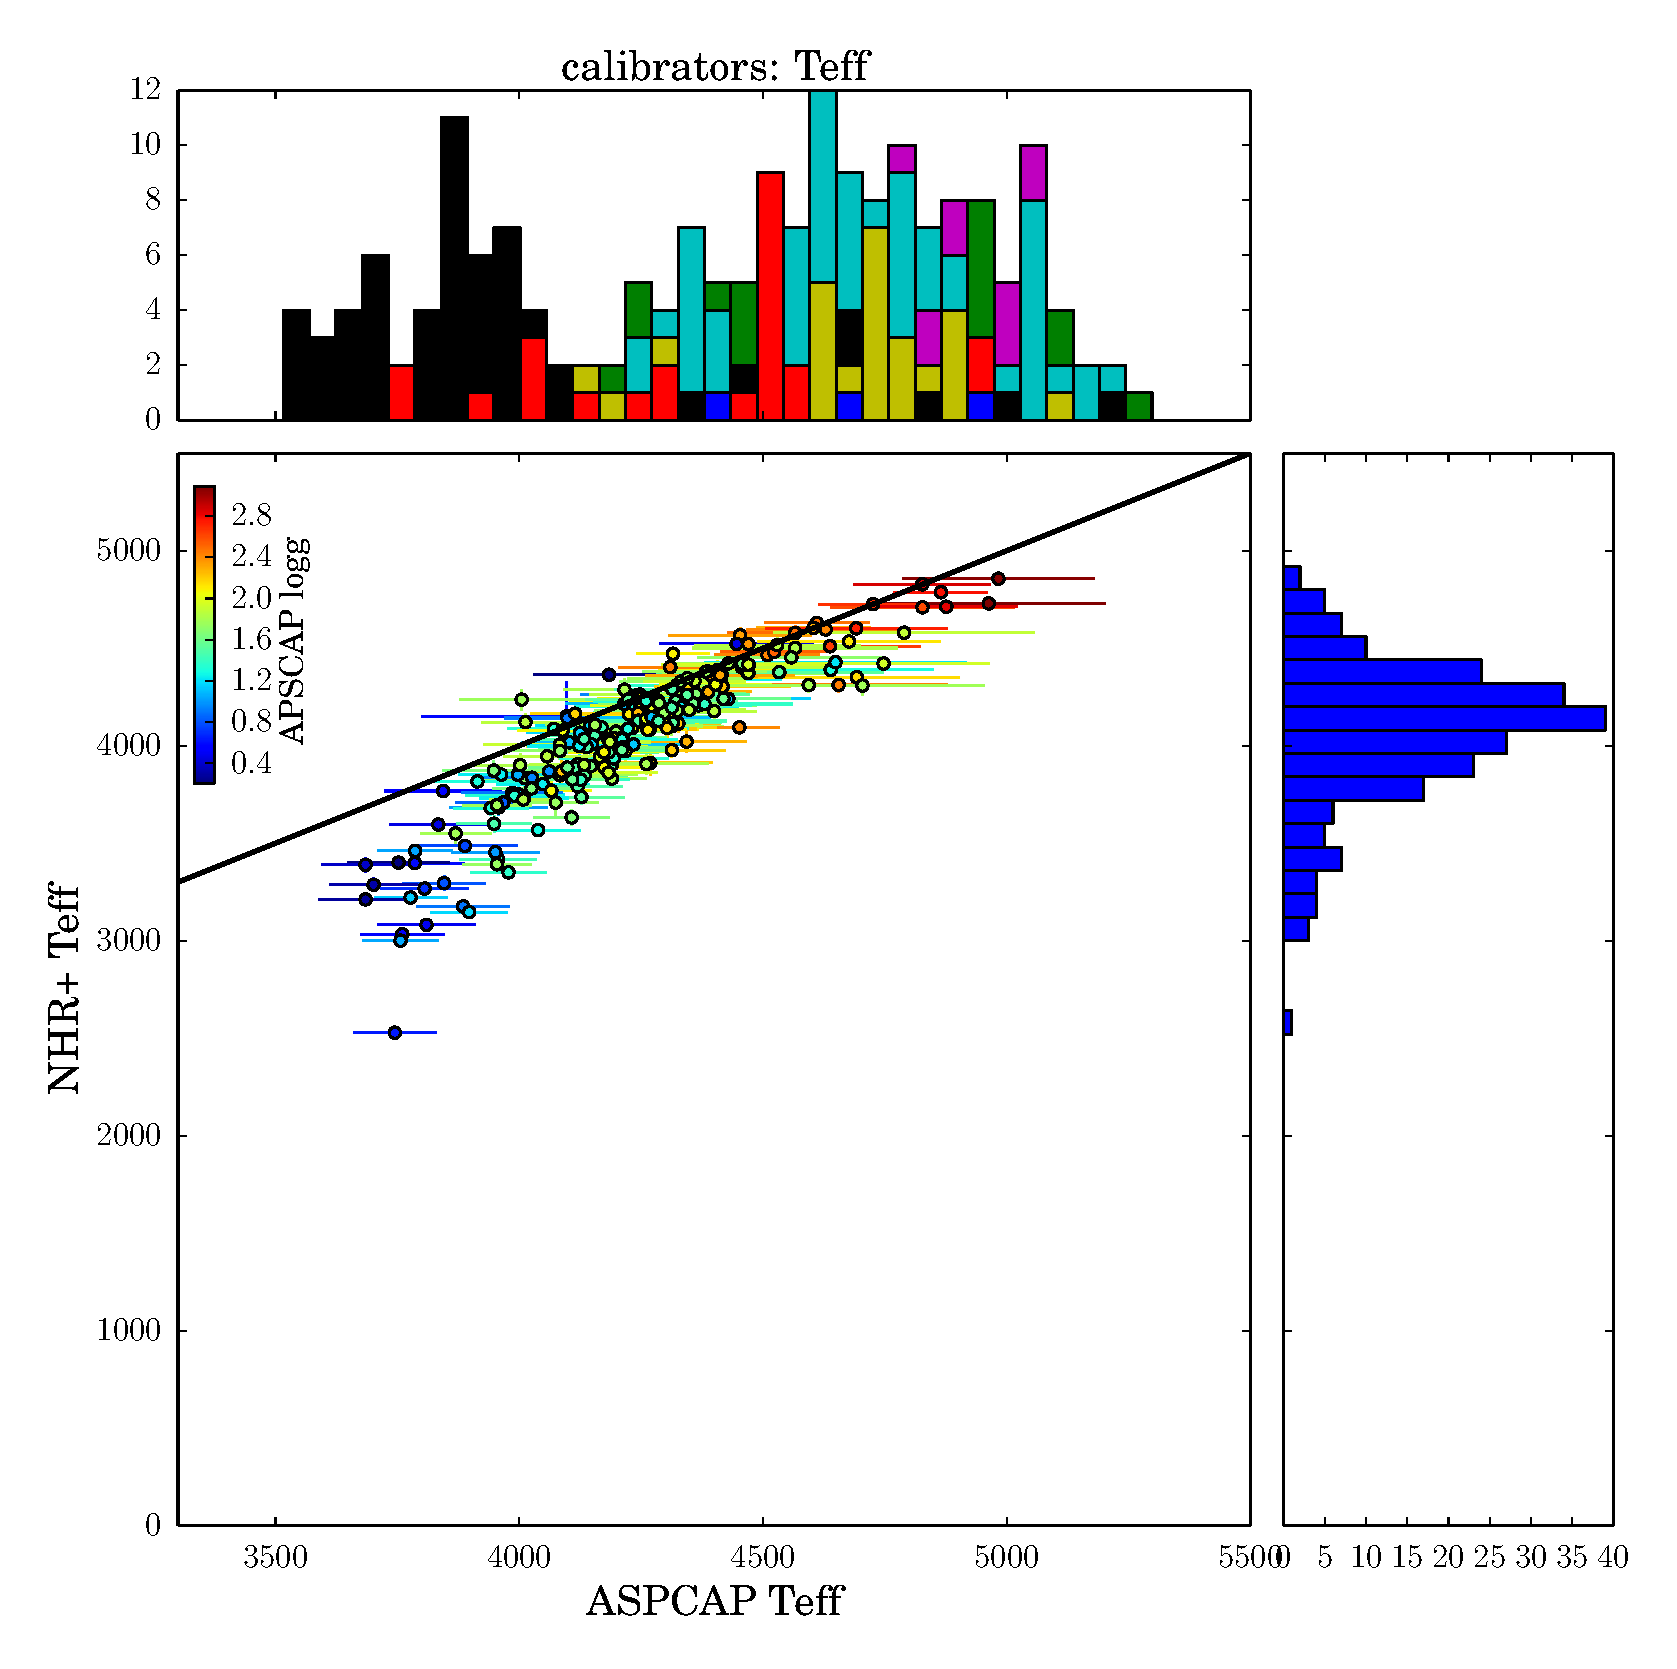
\includegraphics[width=\hsize]{./plots/cal_teff.eps}
\caption{Showing the spread of calibration stars in training set across Teff. Add error bars to these 3 figures showing the calibration.  put colourbar inside fig. have legend for the clusters as well.  }
\label{fig:cal_teff}
\end{figure}

\begin{figure}[h!]
  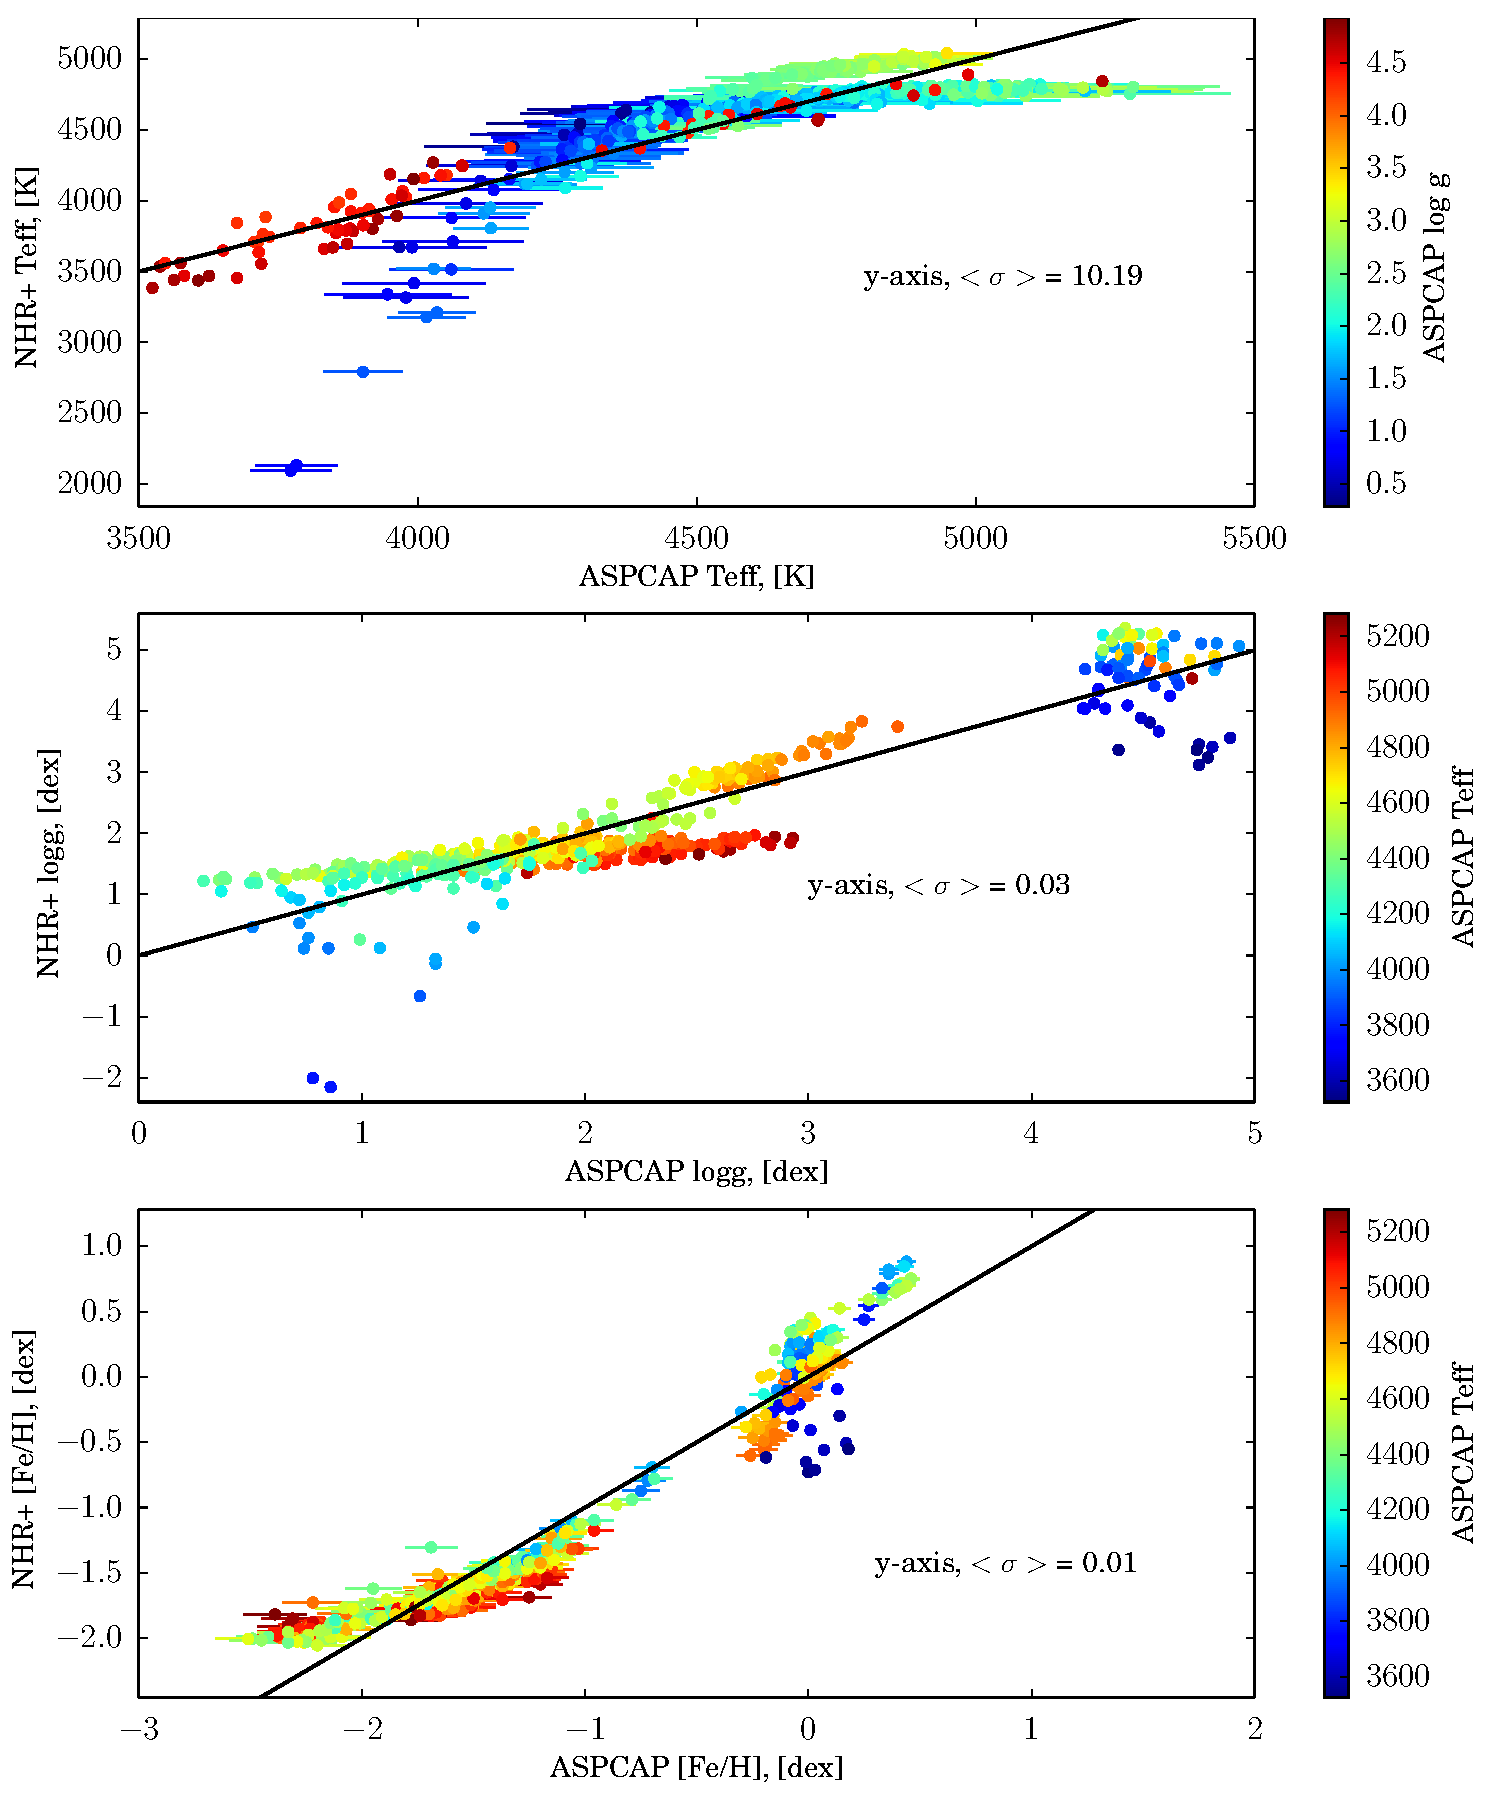
\includegraphics[width=\hsize]{./plots/fits_all3_self.eps}
\caption{this is not a cross validation this is the results of the training set run back through the code. }
\label{fig:cal_teff}
\end{figure}

\begin{figure}[h!]
  \includegraphics[width=\hsize]{./plots/linear_self.png}
\caption{this is not a cross validation this is the results of the training set run back through the code. }
\label{fig:cal_teff}
\end{figure}

\begin{figure}[h!]
  \includegraphics[width=\hsize]{./plots/nonlinear_self.png}
\caption{this is not a cross validation this is the results of the training set run back through the code. }
\label{fig:cal_teff}
\end{figure}

\begin{figure}[h!]
  \includegraphics[width=\hsize]{./plots/4332_all.png}
\caption{this is not a cross validation this is the results of the training set run back through the code. }
\label{fig:cal_teff}
\end{figure}

\begin{figure}[h!]
  \includegraphics[width=\hsize]{./plots/Field_4332_nonlinear.png}
\caption{this is not a cross validation this is the results of the training set run back through the code. }
\label{fig:cal_teff}
\end{figure}

\end{document}
